\setcounter{chapter}{1}
\renewcommand\thechapter{\Alph{chapter}}

\chapter*{Додатки}\addcontentsline{toc}{chapter}{Додатки}

% Styling setup begin
\centeredsection

% Ну и костыль, конечно
% Но когда требуется формативание инвалида - без костылей не обойтись (но это не точно :D )
% \captionsetup[figure]{labelsep=hyphen, justification=centering}

% Styling setup end

\section*{Додаток А}\addcontentsline{toc}{section}{Додаток А}
\begin{center}
	\bfseries Приклади інтерфейсу користувача
\end{center}

\begin{figure}[H]
	\centering
	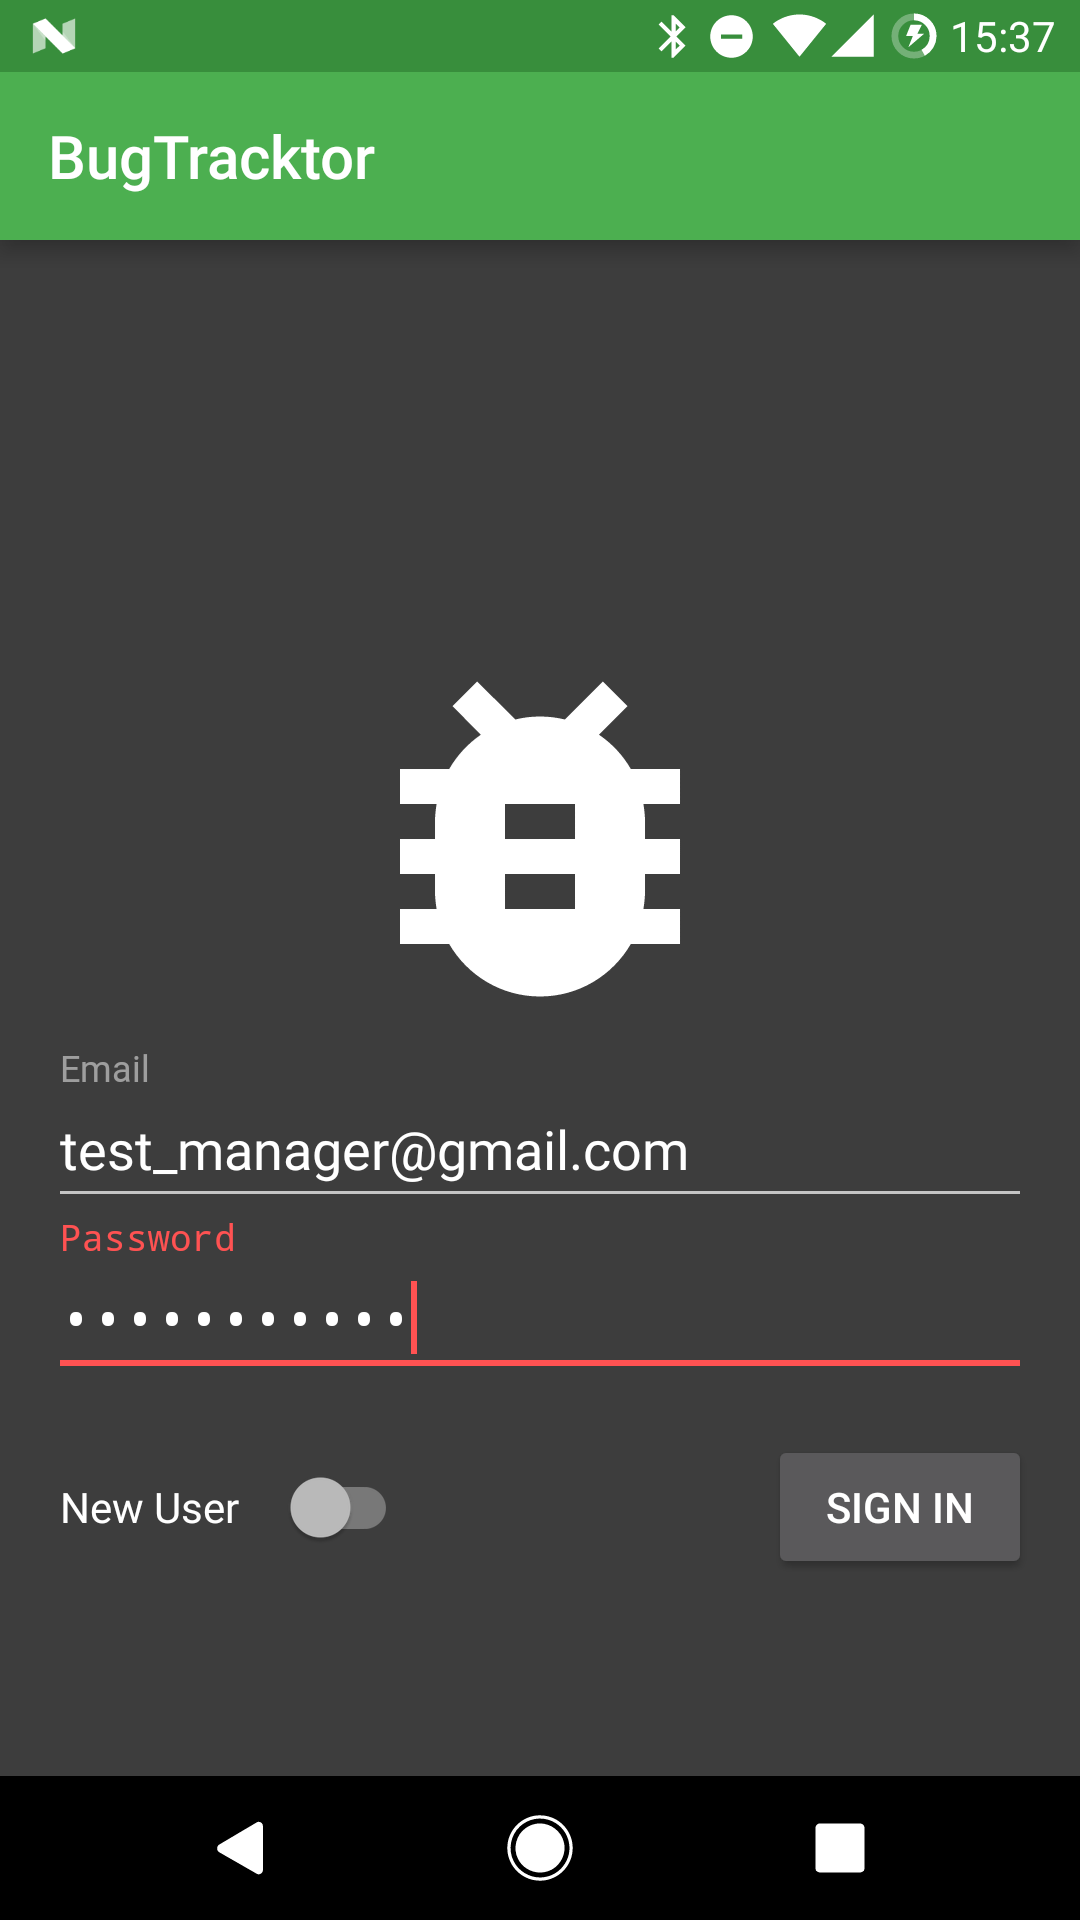
\includegraphics[width=0.6\textwidth]{ui_1}
	\caption{Екран авторизації/реєстрації (авторизація)}
	\label{scr_ui_auth}
\end{figure}

\begin{figure}[H]
	\centering
	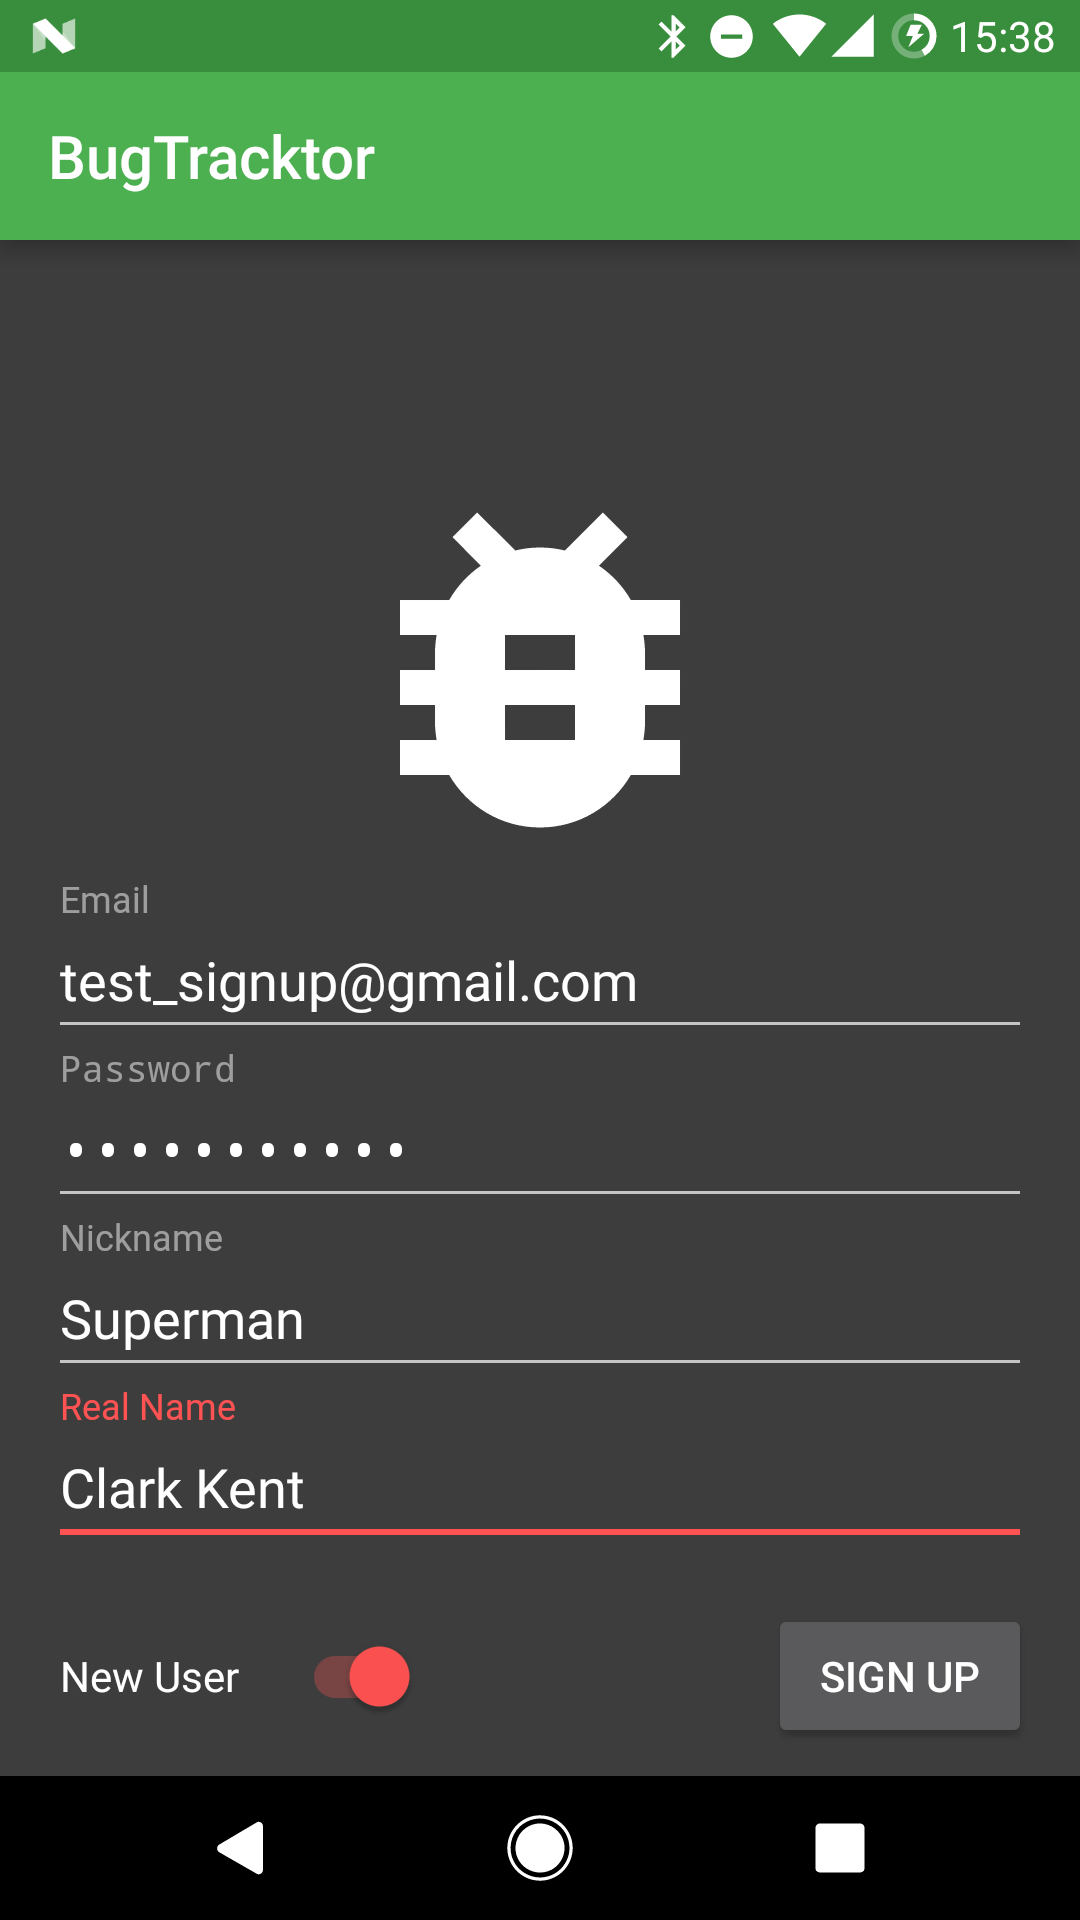
\includegraphics[width=0.75\textwidth]{ui_2}
	\caption{Екран авторизації/реєстрації (реєстрація)}
	\label{scr_ui_signup}
\end{figure}

\begin{figure}[H]
	\centering
	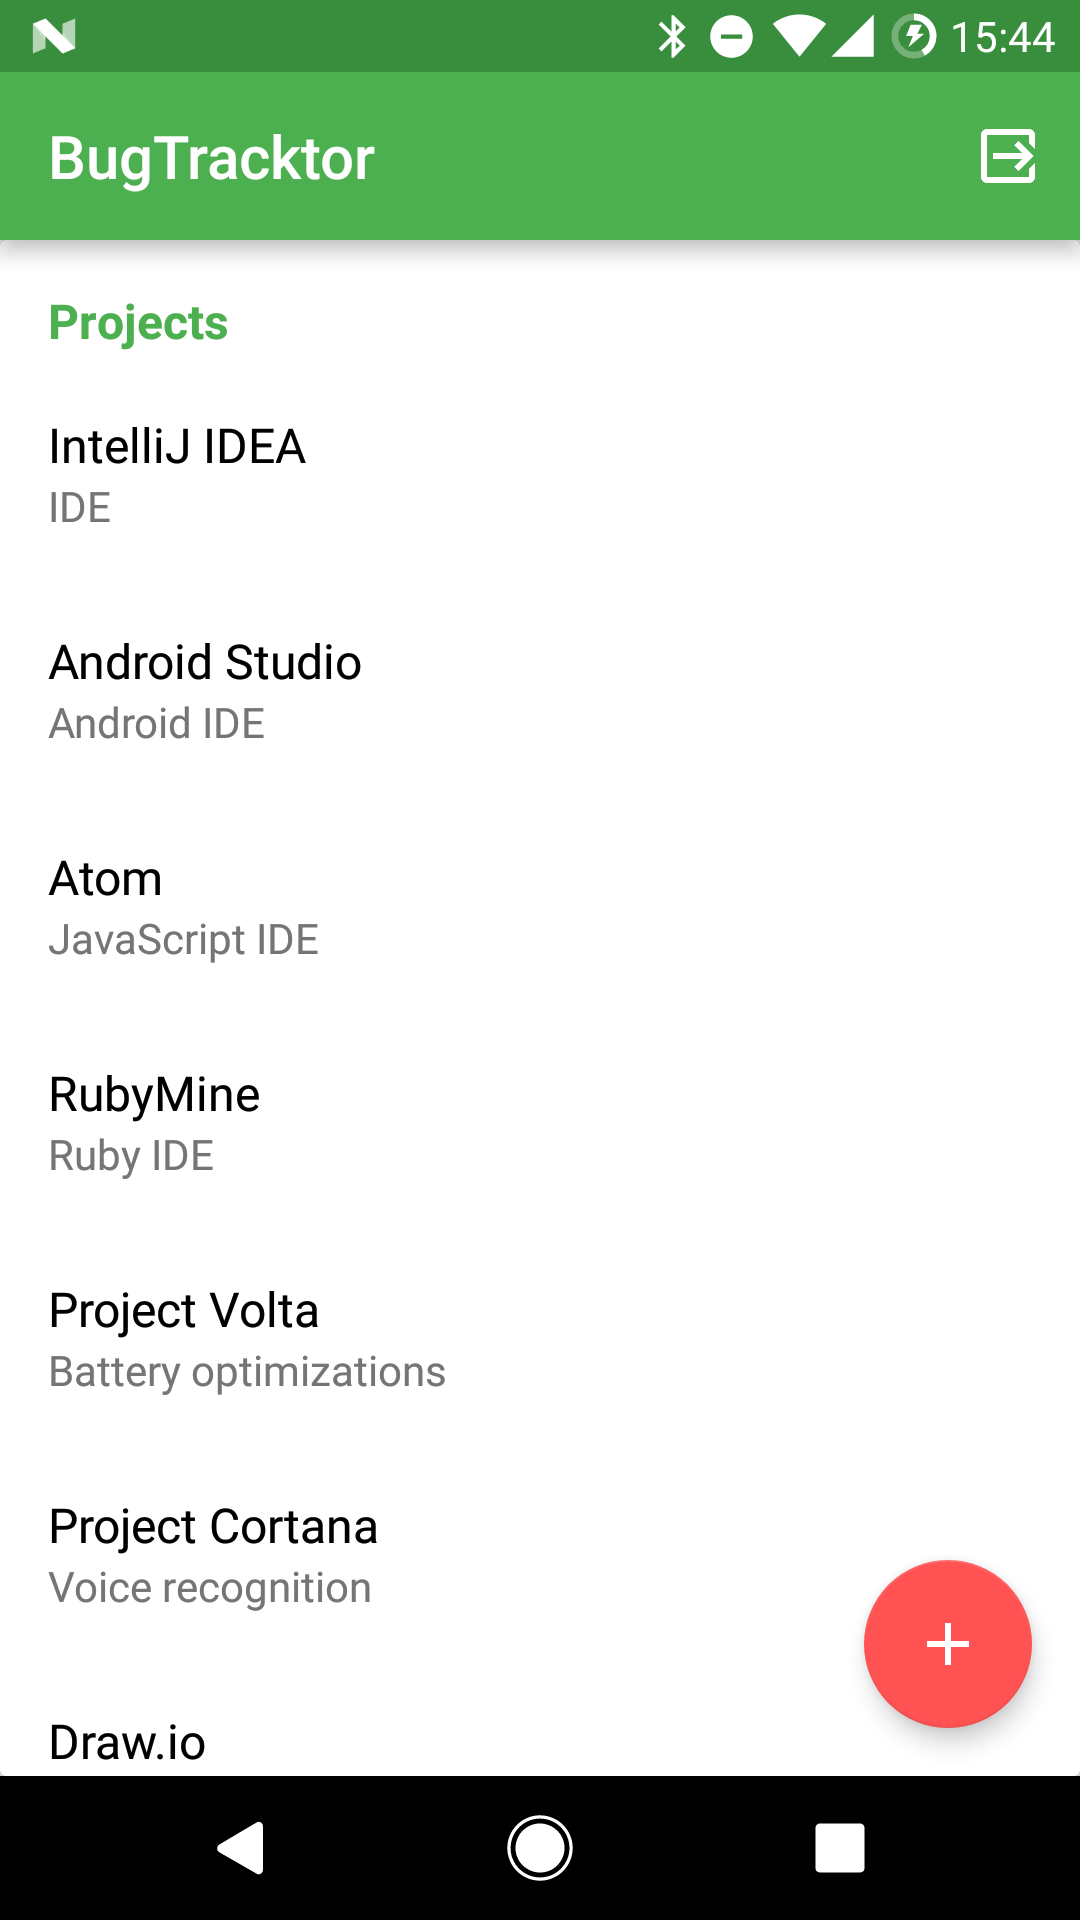
\includegraphics[width=0.75\textwidth]{ui_3}
	\caption{Екран списку проектів}
	\label{scr_ui_projects_list}
\end{figure}

\begin{figure}[H]
	\centering
	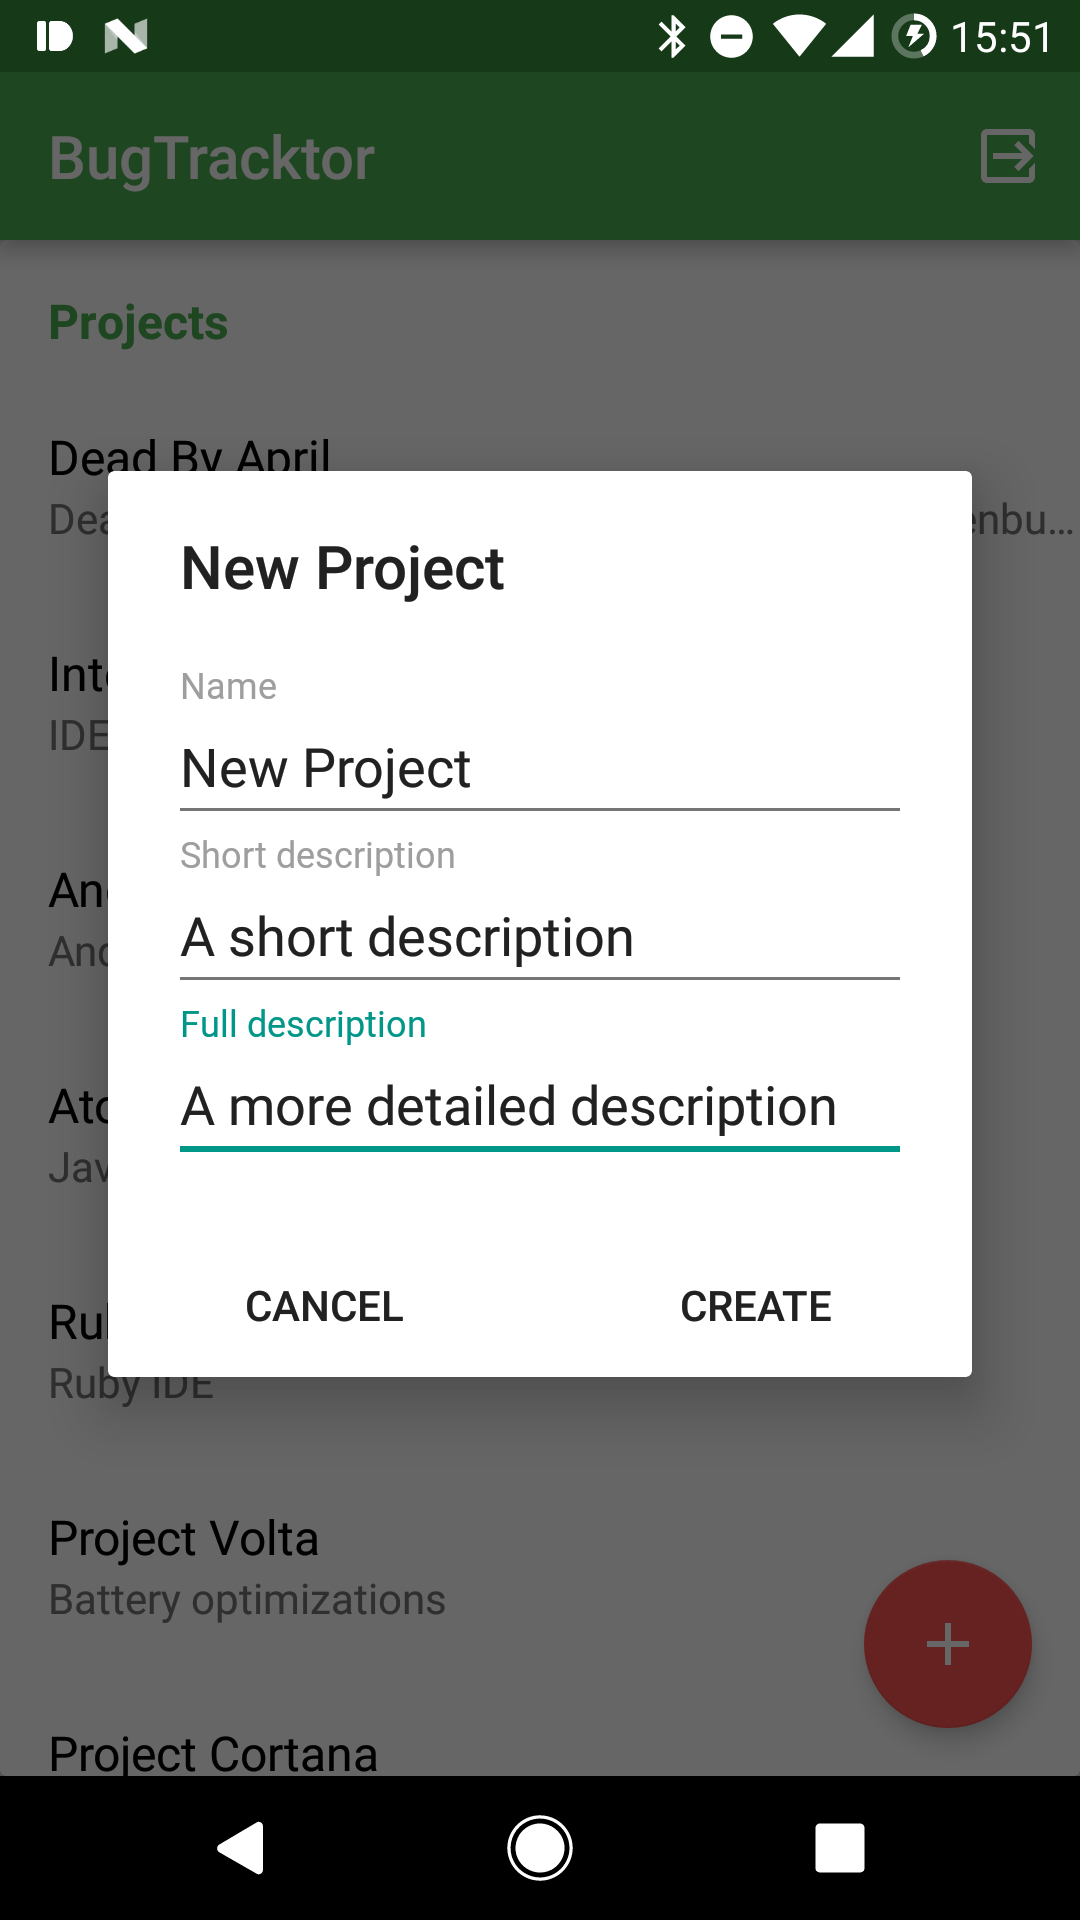
\includegraphics[width=0.75\textwidth]{ui_4}
	\caption{Екран списку проектів}
	\label{scr_ui_project_creation}
\end{figure}

\begin{figure}[H]
	\centering
	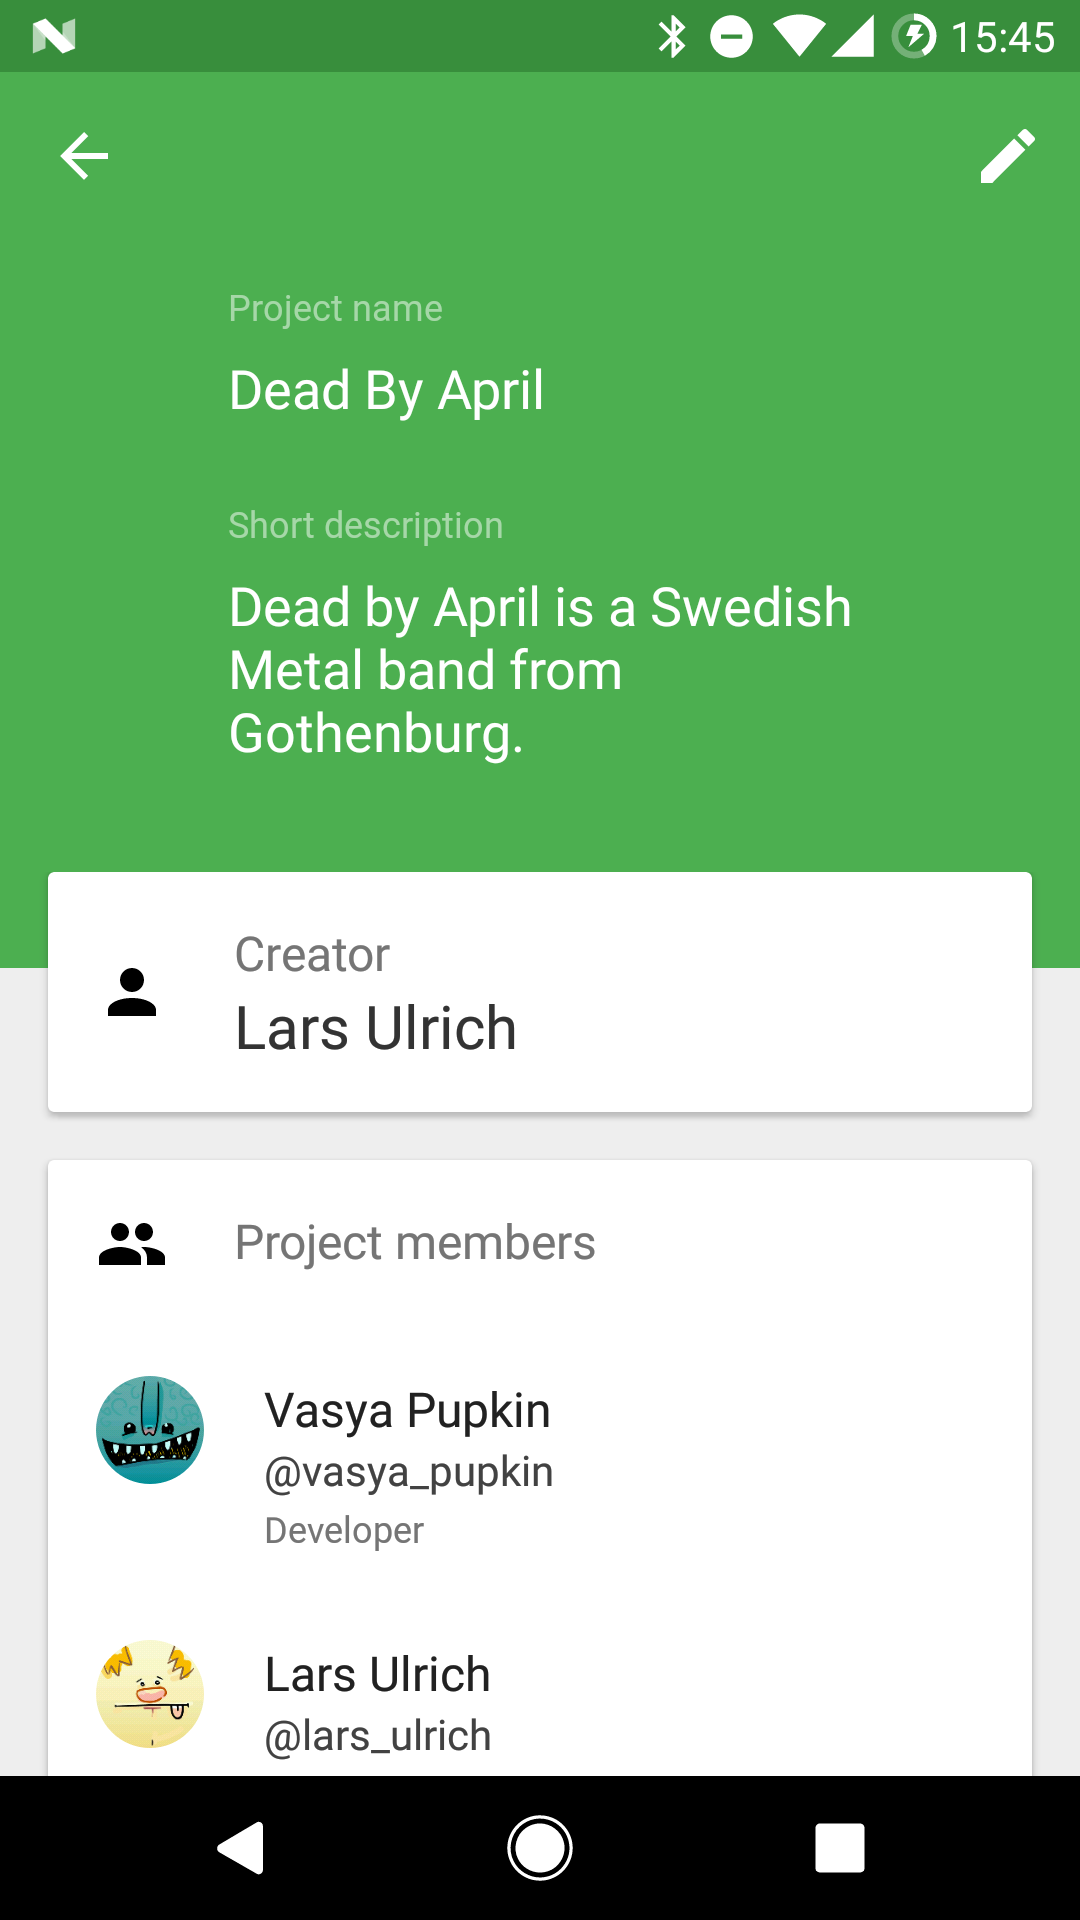
\includegraphics[width=0.75\textwidth]{ui_5}
	\caption{Екран проекту (1)}
	\label{scr_ui_project_1}
\end{figure}

\begin{figure}[H]
	\centering
	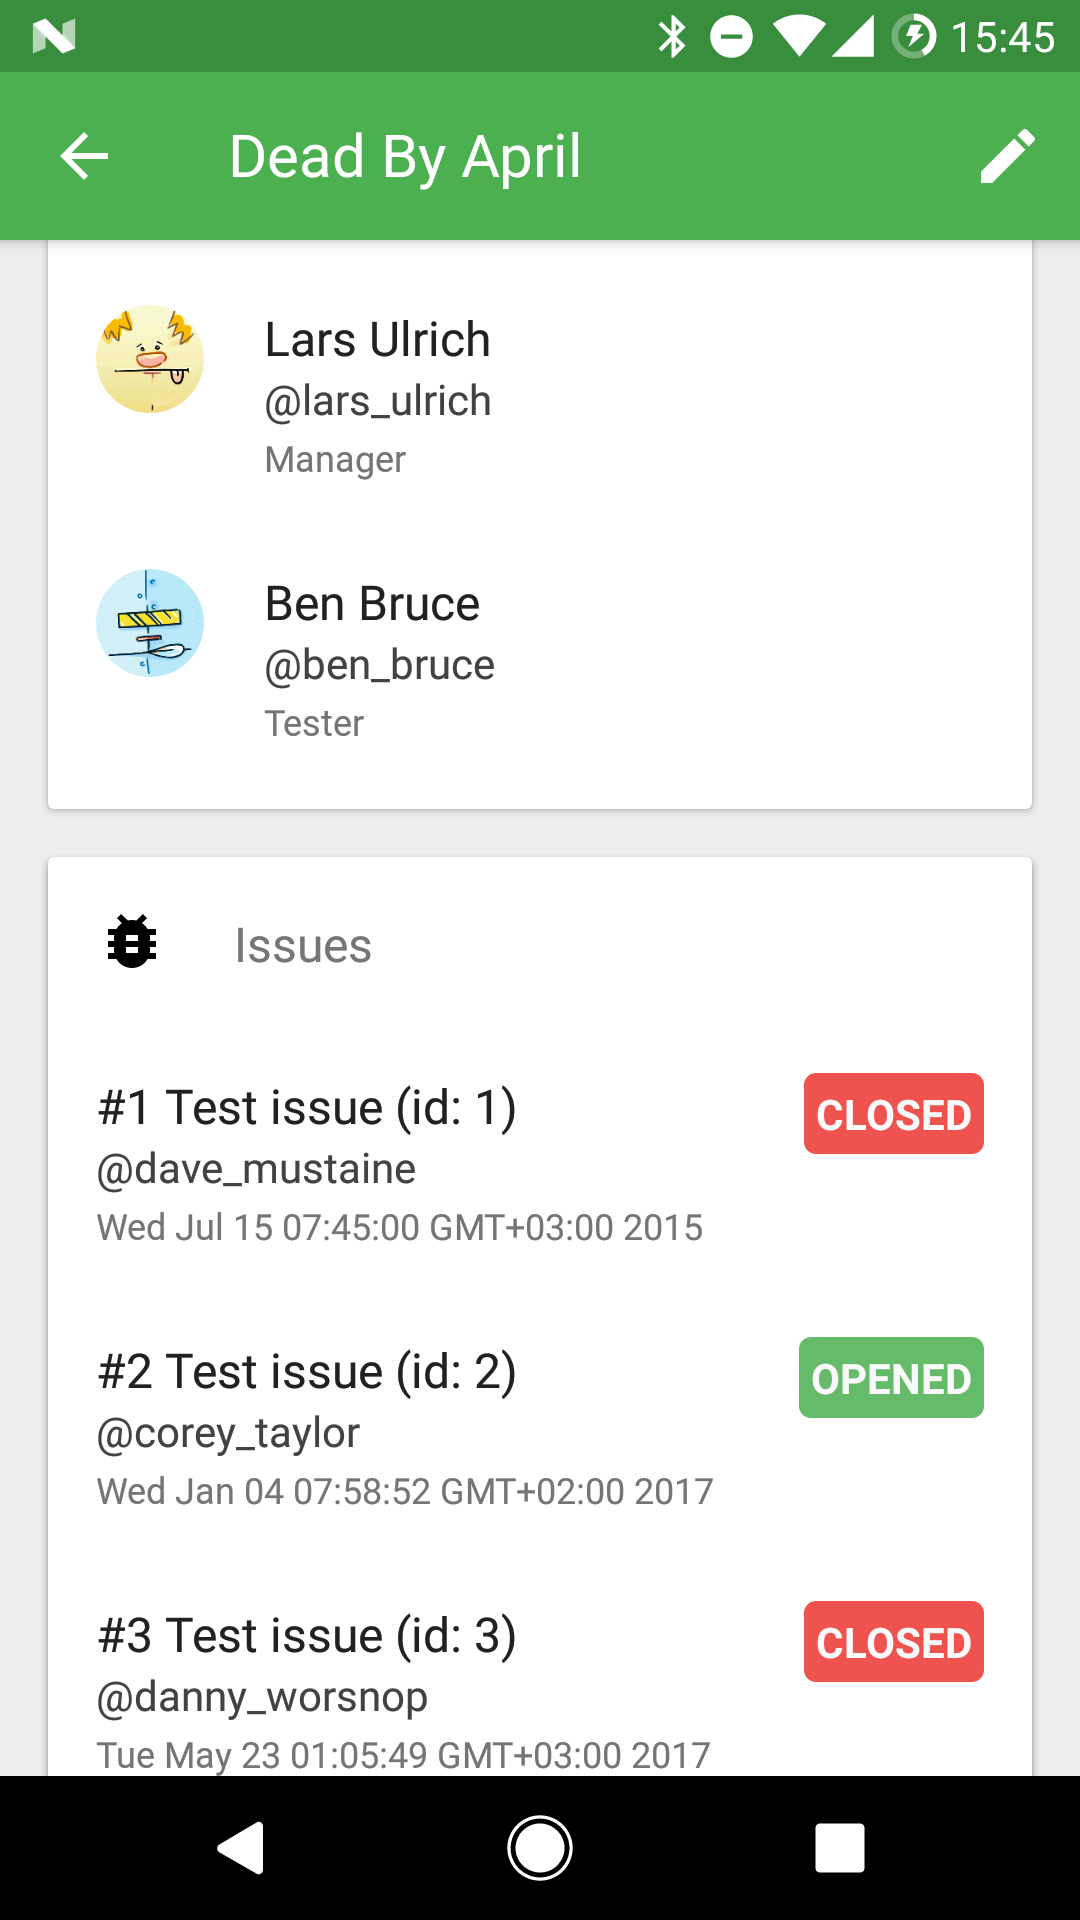
\includegraphics[width=0.75\textwidth]{ui_6}
	\caption{Екран проекту (2)}
	\label{scr_ui_project_2}
\end{figure}

\begin{figure}[H]
	\centering
	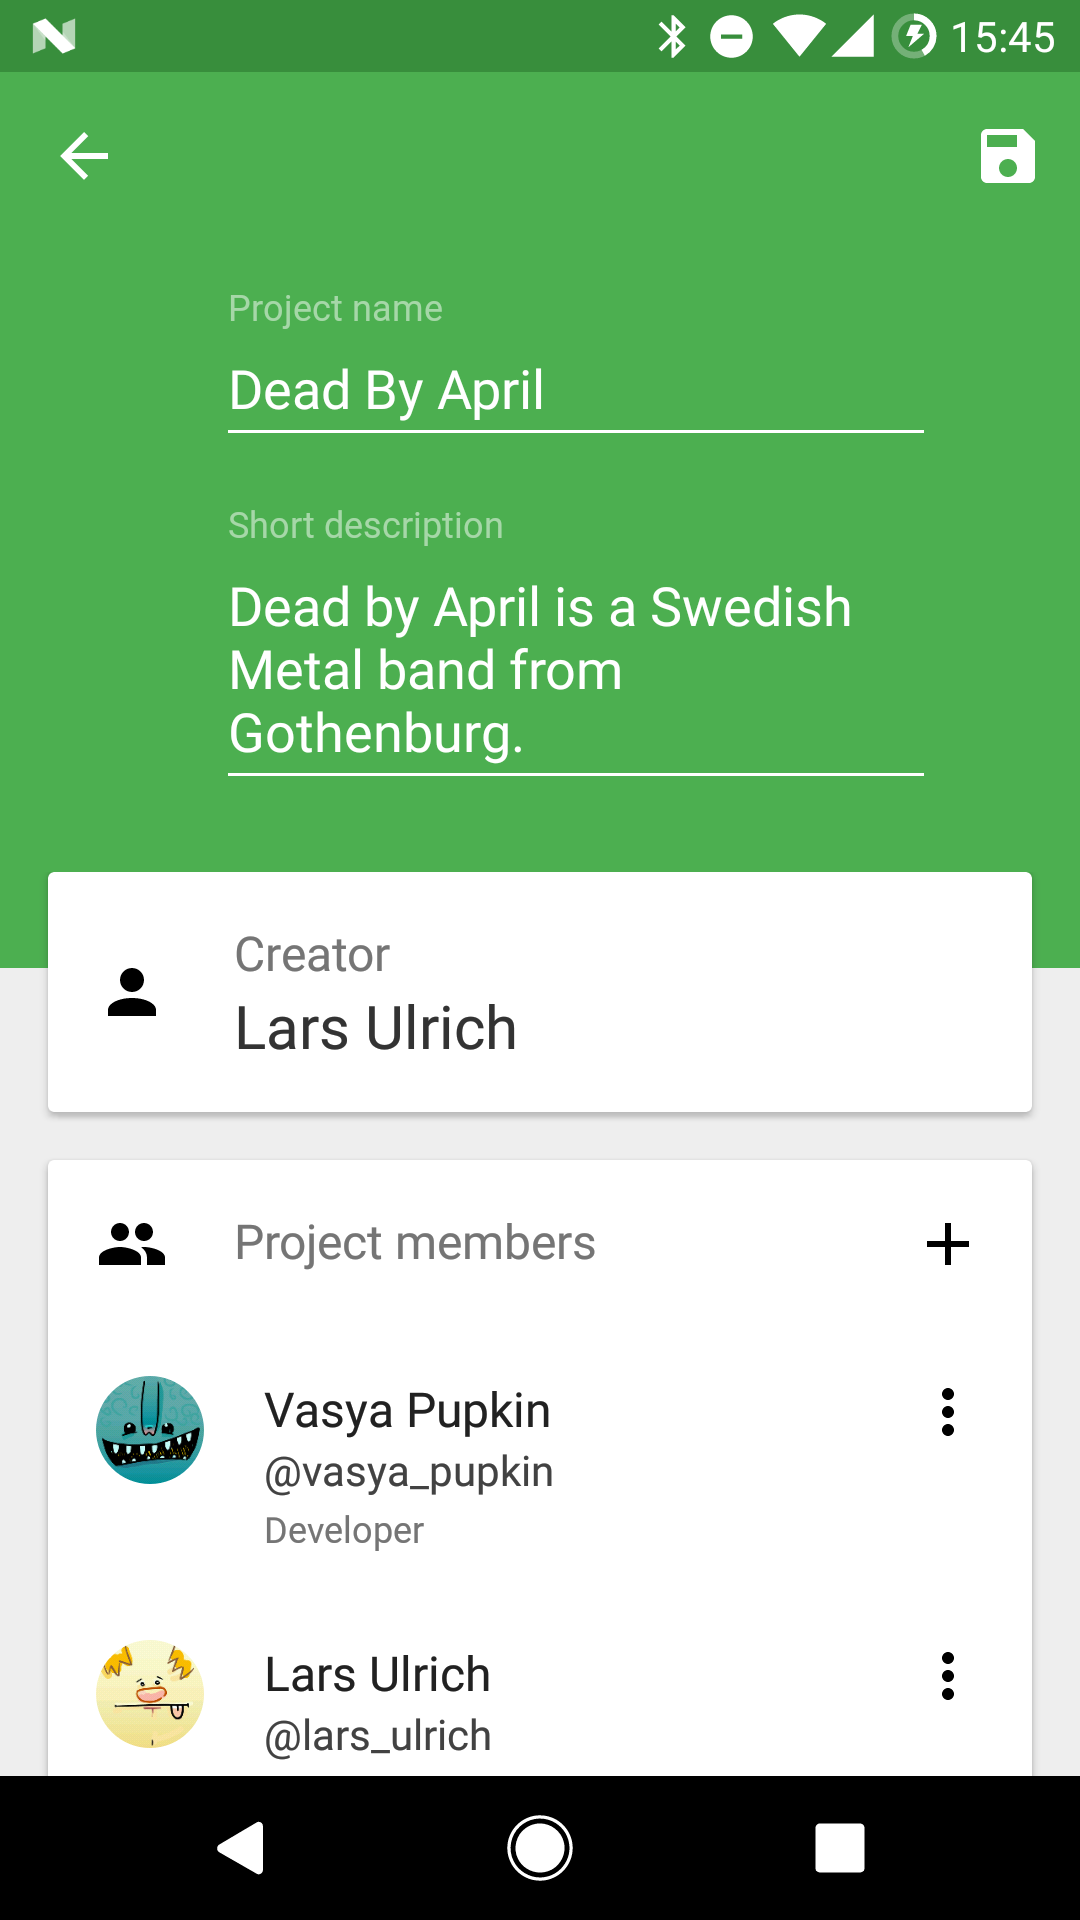
\includegraphics[width=0.75\textwidth]{ui_7}
	\caption{Екран проекту (редагування)}
	\label{scr_ui_project_edit}
\end{figure}

\begin{figure}[H]
	\centering
	
\includegraphics[width=0.75\textwidth]{ui_8}
	\caption{Екран додавання учасника проекту (1 етап).}
	\label{scr_ui_add_project_members_1}
\end{figure}

\begin{figure}[H]
	\centering
	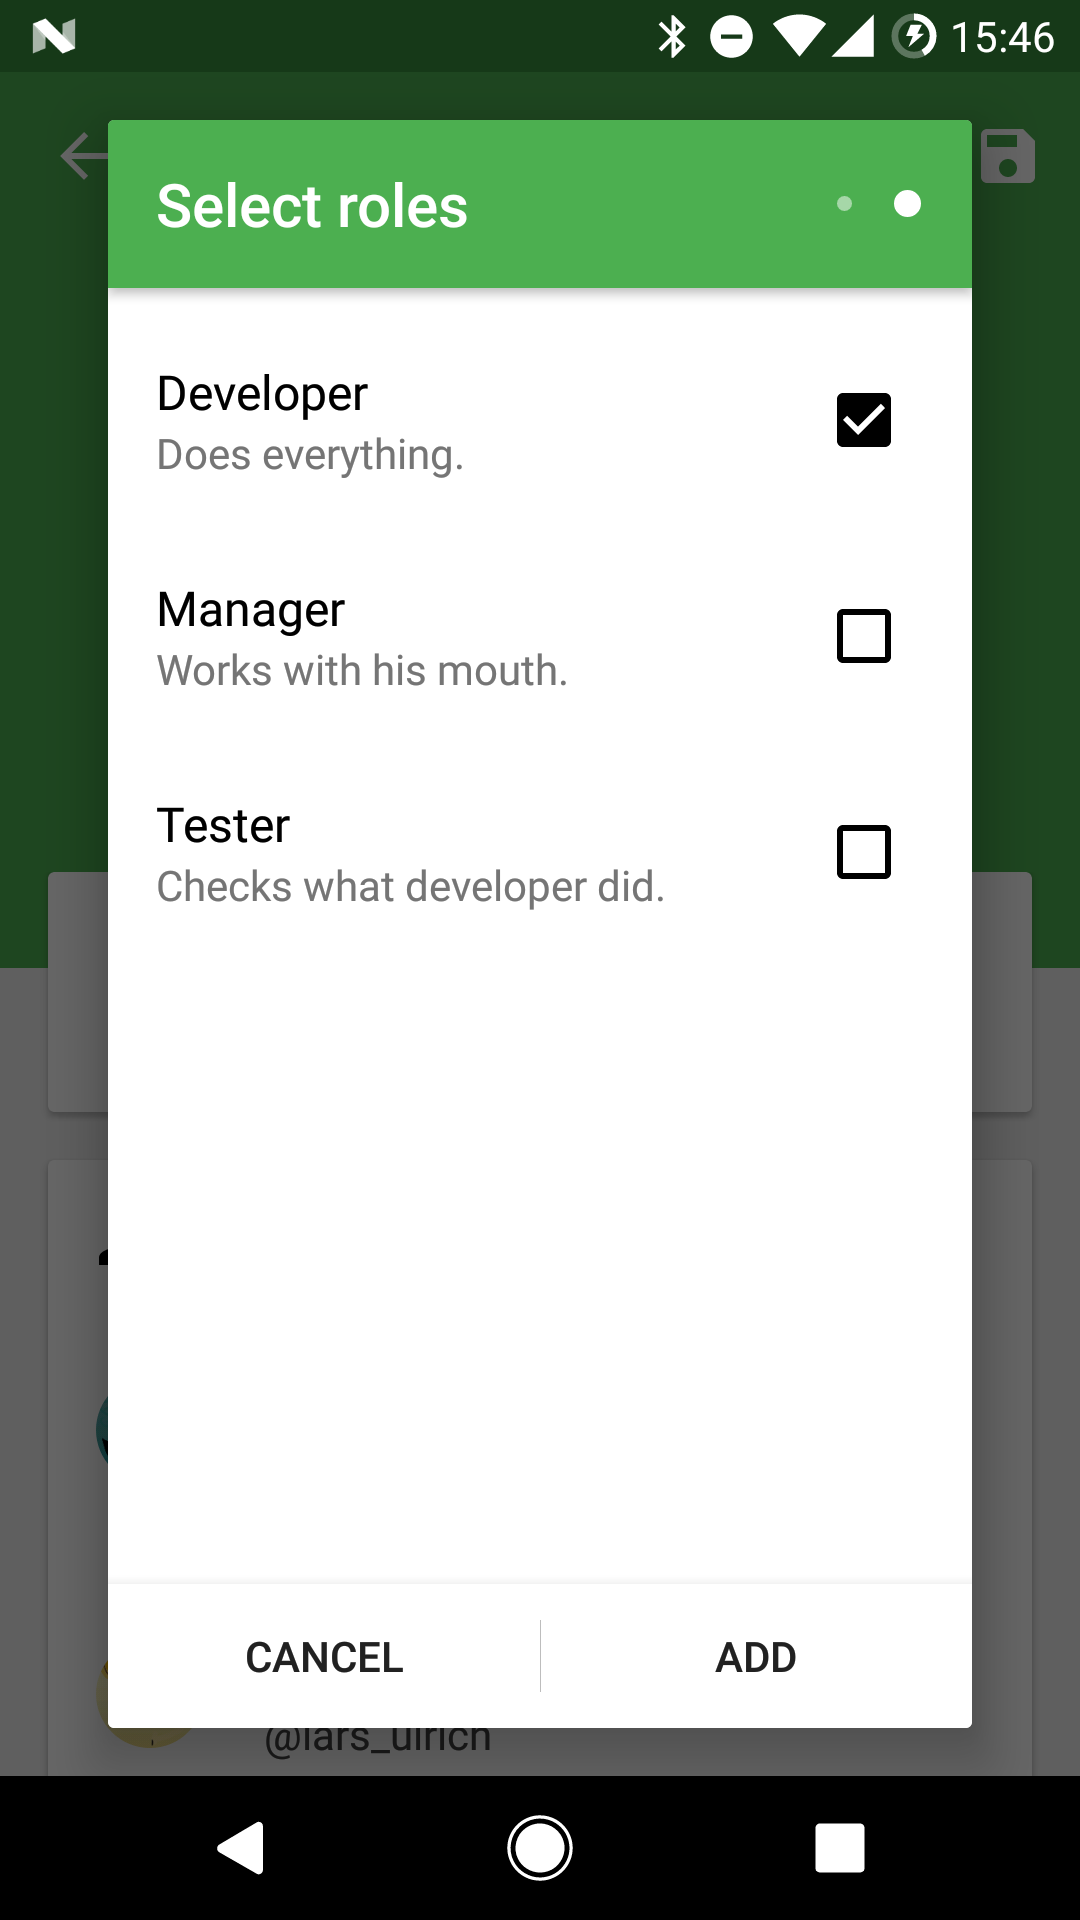
\includegraphics[width=0.75\textwidth]{ui_9}
	\caption{Екран додавання учасника проекту (2 етап).}
	\label{scr_ui_add_project_members_2}
\end{figure}

\begin{figure}[H]
	\centering
	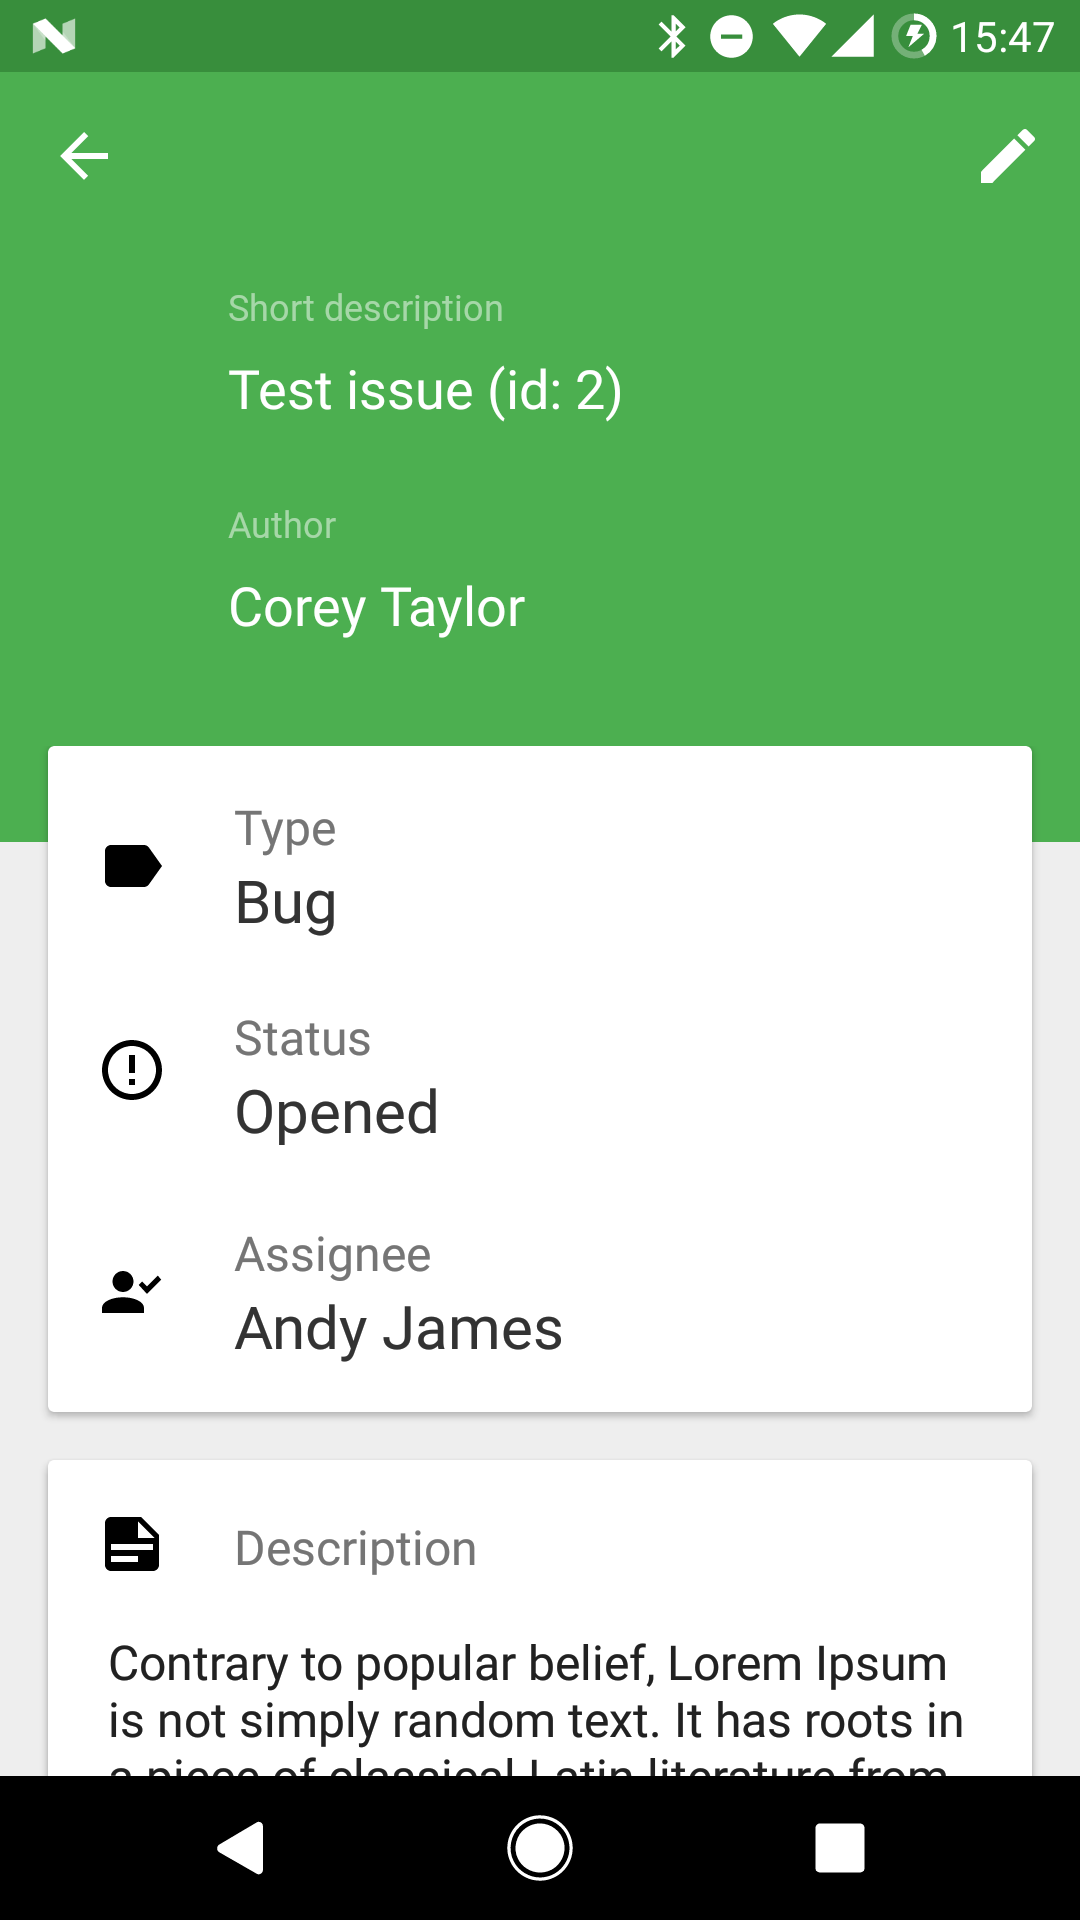
\includegraphics[width=0.75\textwidth]{ui_10}
	\caption{Екран звіту (1).}
	\label{scr_ui_issue_1}
\end{figure}

\begin{figure}[H]
	\centering
	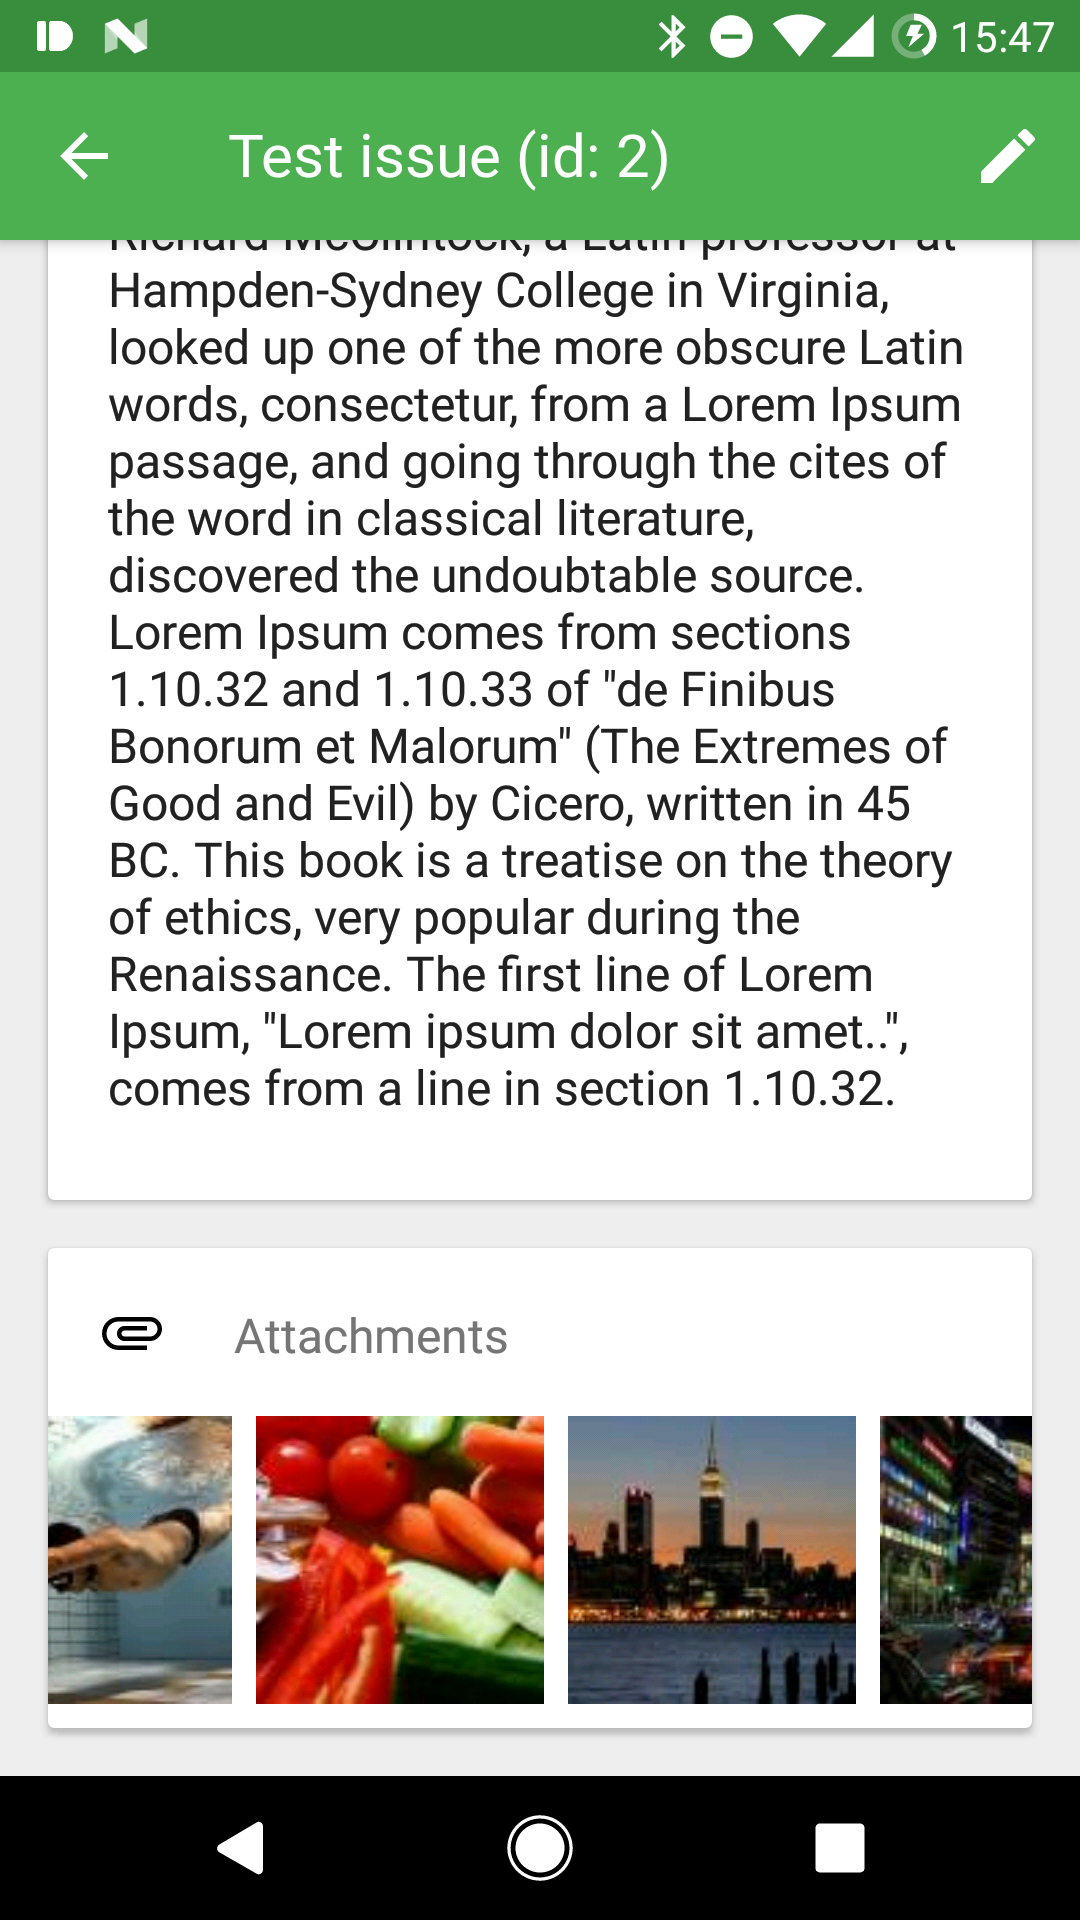
\includegraphics[width=0.75\textwidth]{ui_11}
	\caption{Екран звіту (2).}
	\label{scr_ui_issue_2}
\end{figure}

\begin{figure}[H]
	\centering
	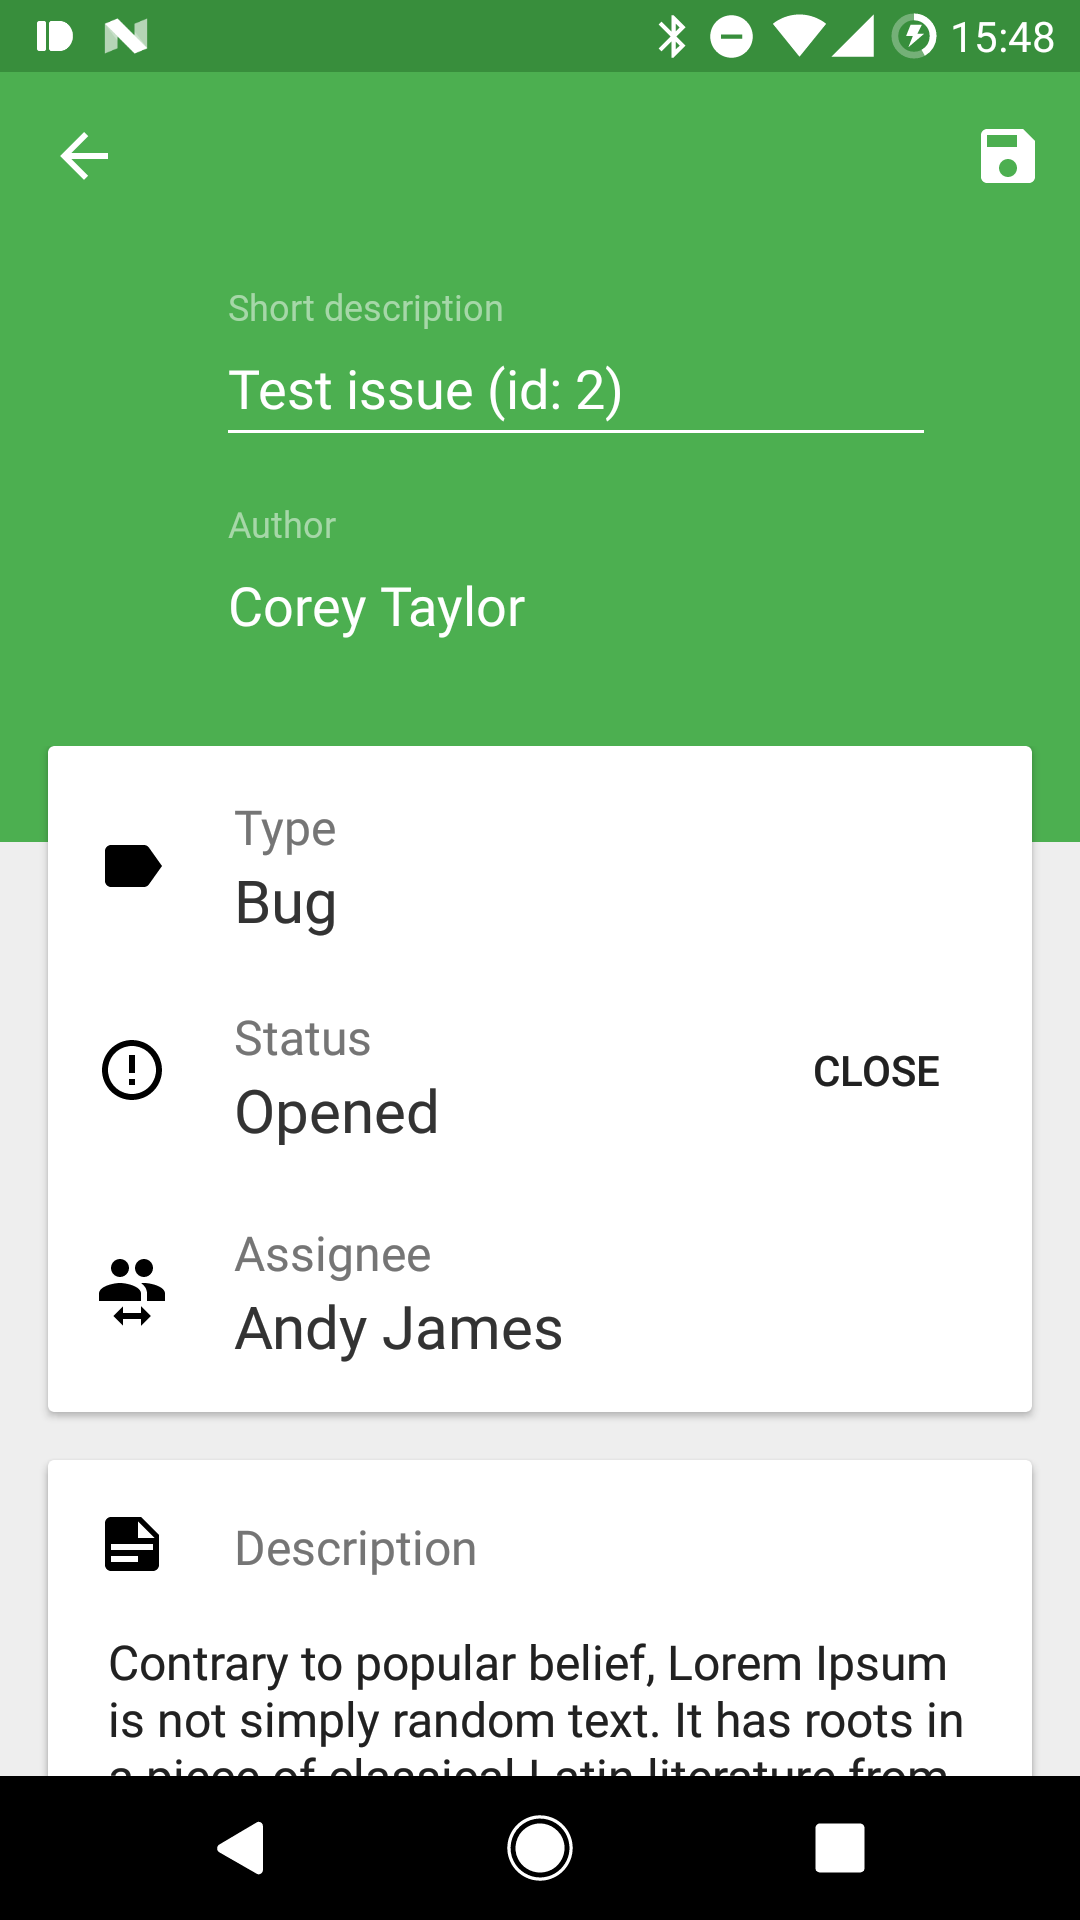
\includegraphics[width=0.75\textwidth]{ui_12}
	\caption{Екран редагування звіту.}
	\label{scr_ui_issue_edit}
\end{figure}